\documentclass{standalone}
\usepackage{tikz}
\usetikzlibrary{calc, positioning, arrows.meta}

\begin{document}
\begin{tikzpicture}[
  msg/.style = {>=Stealth, <->, very thick}]
  \node (ms) [] {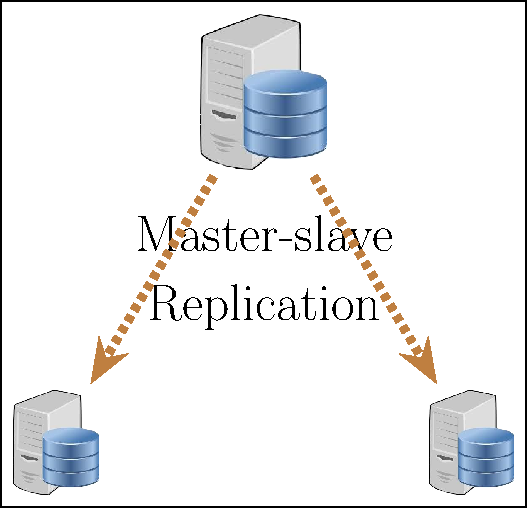
\includegraphics[scale = 0.40]{figs/master-slave.pdf}};
  \node (client) [above = 2.0cm of ms] {
\includegraphics[scale = 0.25]{figs/client-pc-logo.png}};

  % begin
  \draw [msg] (client) to node () [below = 5pt, midway, sloped] {\textsc{Begin}} 
  node () [above = 5pt, midway, sloped] {$T$.sts} (ms);

  % read
  \draw [msg] (client) to [bend right = 40] node () [above = 5pt, midway, sloped] {\textsc{Read}} ($(ms.south west) + (0,20pt)$);

  % write
  \draw [msg] (client) to [out = -30, in = 30, looseness = 5] node () [] {\textsc{Write}} (client);

  % commit
  \draw [msg] (client) to [bend left = 45] node () [below = 5pt, midway, sloped] {\textsc{Commit}} ($(ms.north) + (25pt, 0)$);

  % vc
  \node () [below right = 0.10cm and 0.20cm of client.south, red] {$\textsc{ADD-VC}$};
  \node () [below right = 0.50cm and 0.20cm of ms.north, red] {\textsc{CHECK-VC}};
\end{tikzpicture}
\end{document}